% p10-05 例 3：正方形 ABCD 边长 6, E∈CD, F∈BC，沿 AE 折 △ADE 使 D→D'，沿 AF 折 △ABF 使 B→B'，D'=B'=P∈AC.
% 由 ∠DAE=∠BAF=22.5°，DE=BF=6 tan22.5° = 6(√2-1)≈2.485
% A(0,6), B(6,6), C(6,0), D(0,0) —— 让 AC 为对角线
% 改设 A(0,0), B(6,0), C(6,6), D(0,6)；AC 从 (0,0) 到 (6,6)
\documentclass[tikz,border=4pt]{standalone}
\usepackage{ctex}
\usepackage{amsmath}
\usetikzlibrary{calc}
\begin{document}
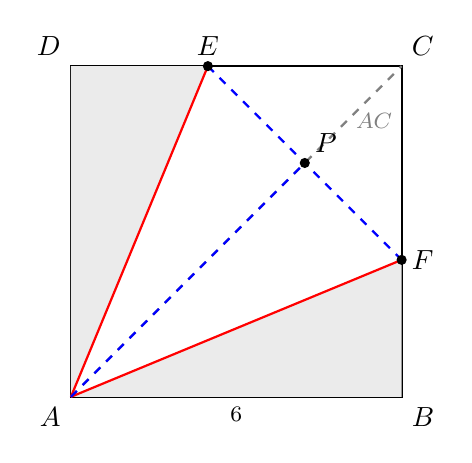
\begin{tikzpicture}[scale=0.7, thick]
  \coordinate (A) at (0,0);
  \coordinate (B) at (6,0);
  \coordinate (C) at (6,6);
  \coordinate (D) at (0,6);
  % DE = 6(√2-1) ≈ 2.485 沿 DC 方向；E ∈ CD = 上边
  % CD 从 C(6,6) 到 D(0,6)，DE 从 D(0,6) 沿 DC 方向 = (1,0): E = (2.485, 6)
  \coordinate (E) at (2.485, 6);
  % BF = 6(√2-1) ≈ 2.485 沿 BC 方向；F ∈ BC = 右边；BF 从 B(6,0) 向 C(6,6): F=(6, 2.485)
  \coordinate (F) at (6, 2.485);
  % P 在 AC 上，AP = 6: P = (6/√2)(1,1) = (4.243, 4.243)
  \coordinate (P) at (4.243, 4.243);

  \draw (A)--(B)--(C)--(D)--cycle;
  \draw[gray, dashed] (A)--(C);   % 对角线

  % 折前 △ADE 灰色填充
  \fill[black!8] (A)--(D)--(E)--cycle;
  % 折前 △ABF
  \fill[black!8] (A)--(B)--(F)--cycle;
  % 折后 △AP（D'=P）与 △AP（B'=P）共点 P
  \draw[red, thick] (A)--(E);     % 折痕 AE
  \draw[red, thick] (A)--(F);     % 折痕 AF
  \draw[blue, dashed, thick] (A)--(P);    % AD' = AB' = AP
  \draw[blue, dashed, thick] (E)--(P);    % E→P (D 的对应)
  \draw[blue, dashed, thick] (F)--(P);    % F→P (B 的对应)

  \filldraw (E) circle (2pt);
  \filldraw (F) circle (2pt);
  \filldraw (P) circle (2pt);

  \node[below left]  at (A) {$A$};
  \node[below right] at (B) {$B$};
  \node[above right] at (C) {$C$};
  \node[above left]  at (D) {$D$};
  \node[above] at (E) {$E$};
  \node[right] at (F) {$F$};
  \node[above right] at (P) {$P$};

  \node[below] at ($(A)!0.5!(B)$) {\footnotesize $6$};
  \node[font=\footnotesize, gray] at (5.5, 5.0) {$AC$};
\end{tikzpicture}
\end{document}
